\documentclass[12pt]{article}
\usepackage{graphicx}
\usepackage{hyperref}
\usepackage{eso-pic} 
\usepackage{lipsum} 
\usepackage{amsmath}
\usepackage{listings}
\usepackage{amsmath}
\usepackage[linesnumbered,ruled, longend]{algorithm2e}
\usepackage{tikz}
\usepackage{tabularx}
\usepackage{colortbl}
\usepackage{fancyhdr}
\usepackage{float}
\usepackage{xcolor}
\usepackage[T1]{fontenc}

\usetikzlibrary{shapes.geometric, arrows}
\tikzstyle{node} = [rectangle, rounded corners, minimum width=1cm, minimum height=1cm,text centered, text width=3cm, draw=black, fill=red!30]
\tikzstyle{level1} = [rectangle, rounded corners, minimum width=1cm, minimum height=1cm, text centered,text width=3cm, draw=black, fill=orange!30]
\tikzstyle{level2} = [rectangle, rounded corners, minimum width=1cm, minimum height=1cm, text centered,text width=3cm, draw=black, fill=green!30]
\tikzstyle{level3} = [rectangle, rounded corners, minimum width=1cm, minimum height=1cm, text centered,text width=1.5cm, draw=black, fill=blue!30]
\tikzstyle{arrow} = [thick,->,>=stealth,blue]
\tikzset{edge from parent path={ (\tikzparentnode) -- +(0,-20pt) -| (\tikzchildnode)}}
%%%%%%%%%%%%%%%%%%%%%%%%%%%%%%%%%%%%%%%%%%%%%%%%%%%%%%%%%%%%%%%%%%%%%%%%%%
\setlength{\parindent}{0em}
\setlength{\parskip}{1em}
%%%%%%%%%%%%%%%%%%%%%%%%%%%%%%%%%%%%%%%%%%%%%%%%%%%%%%%%%%%%%%%%%%%%%%%%%%
\definecolor{pblue}{rgb}{0.13,0.13,1}
\definecolor{pgreen}{rgb}{0,0.5,0}
\definecolor{pred}{rgb}{0.9,0,0}
\definecolor{backcolour}{rgb}{0.95,0.95,0.92}
\lstset{language=Java,
	backgroundcolor=\color{backcolour},
	commentstyle=\color{pgreen},
	keywordstyle=\color{pblue},
	stringstyle=\color{pred},
	basicstyle=\ttfamily,
	numbers=left,
	numberstyle=\tiny,
	frame=single,
	title=\lstname
}

\definecolor{bluepale}{RGB}{10,120,155}
%---------------------------------------------


\title{- Rapport Projet - \\Conception Logicielle avancée \\ \textbf{Solveur Robot Ricochet} }
\author{ Erwan Phillipe MENSAH \\ TOURE Papa Samba Khary \\Daouda TRAORE}
\renewcommand*\contentsname{Table des matières}
\date{}
\begin{document}
\AddToShipoutPicture*
{\put(440,650){\includegraphics[width=6cm,height=6cm]{Images/logo.jpg}}}
\maketitle
\mbox{}
\vfill
L2 Informatique 2021-2022 Université Caen Basse-Normandie.

\newpage
\tableofcontents
%%%%%%%%%%%%%%%%%%%%%%%%%%%%%%%%%%%%%%%%%%%%%%%%%%%%%%%%%%%%%%%%%%%%%%%%%%%%%%%%%%%%%%%%
\newpage
\section{Introduction}	
	Dans le cadre de notre second semestre , il nous a été proposé multiples sujets nous permettant de mettre en
	pratique nos connaissances et nos compétences. Parmis tous ces sujets celui qui nous a le plus intéressé fut le \textbf{solver} du jeu de société "\textbf{Ricochet Robots}.
	\\
	Comme c’est le cas pour beaucoup de jeux de société, il est possible d'en réaliser une application. 
	\\
	Le but du projet etait de dévolopper un programme capable de trouver une solution optimale pour toute situation du jeu.
	\\
	Trois objectifs étaient à remplir. Dans un premier temps il faillait développer le \textbf{moteur du jeu} puis d'implémenter un \textbf{algorithme de résolution A*} et de l'optimiser étant
	donné la compléxité du problème et finalement de réaliser une \textbf{interface graphique}.
	\\
	Ce projet nous a donc amené à travailler sur des connaissances qui sont nouvelles pour
	nous, que ce soit les  algorithmes de résolution ou encore des choses complexes du développement des applications. Ce rapport a pour objectif de présenter comment nous avons travaillé et quels ont été les
	multiples obstacles que nous avons du faire face.
	\\
	Le présent rapport est organisé en trois grandes parties. La première est consacrée à la présentation du jeu, puis nous parlerons de la répartition des tâches, du développement du moteur,
	de la réalisation du solveur, enfin de la création  de l'interface graphique et des problèmes rencontrés.
\newpage
%%%%%%%%%%%%%%%%%%%%%%%%%%%%%%%%%%%%%%%%%%%%%%%%%%%%%%%%%%%%%%%%%%%%%%%%%%%%%%%%%%%%%%%	
\section{\underline{Présentation}}
\begin{figure}[h!]
	\begin{center}
		\includegraphics[width=1\textwidth]{Images/plateau.jpeg}
	\end{center}
	\caption{Ricochet Robots}
	\label{plateau}
\end{figure}
	Ricochet robots est un jeu de société pour deux personnes voir plus, imaginé par Alex Randolph. L'objectif du jeu est de déplacer les robots afin d'atteindre la cible en un minimum
	de mouvements possibles avec des restrictions strictes sur les movements des robots. Le jeu fut publier pour la première fois en Allemagne sous le nom de \textbf{Rasende Roboter} en 
	\textbf{1999}.
	\newpage
\begin{figure}[h!]
	\begin{center}
		\includegraphics[width=1\textwidth]{Images/palteau3.jpg}
	\end{center}
	\caption{Dans l’exemple ci-dessus, l’objectif, indiqué par le jeton placé au centre, est la case verte contenant la planète saturne. Tous les joueurs devront donc s’efforcer de trouver en un minimum 
	de coups le moyen de déplacer le Robot vert jusqu'à cette objectif}
	\label{plateau}
\end{figure}
\newpage	

%%%%%%%%%%%%%%%%%%%%%%%%%%%%%%%%%%%%%%%%%%%%%%%%%%%%%%%%%%%%%%%%%%%%%%%%%%%%%%%%%%%%%%%
	\paragraph{\underline{Contenu}	}
	\begin{itemize}
		\item 4 plateaux imprimés sur les deux faces.
		\item 1 pièce centrale en plastique
		\item 4 robots en 4 couleurs.
		\item 4 jetons carrés aux couleurs des robots.
		\item 17 jetons de cible ronds.
		\item 1 sablier (environ 1 minute)
	\end{itemize}
	\paragraph{\underline{Préparatifs}}
	\begin{itemize}
		\item Placez les quatre plateaux avec le coin troué au centre. Il y a 96 façons différentes de poser
		les plateaux. Fixez les plateaux à l’aide de la pièce de blocage en plastique.
		\item Posez au hasard les quatre jetons colorés sur des cases libres. Placez les robots sur les
		carrés de leurs couleurs respectives.
		\item Mélangez les 17 cibles faces cachées sur la table.
		\item Placez le sablier à côté du plateau de jeu. Retournez une cible au hasard et placez-la face
		visible sur la pièce de blocage centrale. Le jeu peut commencer.
	\end{itemize}
	\paragraph{\underline{But du jeu}\\} 
	Lors de chaque tour, le but est de gagner le jeton cible au centre. Sur le plateau, le même dessin
	est représenté une fois, avec le même symbole et la même couleur. C’est la cible du tour. Votre
	but est de trouver comment le robot de même couleur, dit robot actif, peut atteindre cette cible en
	le moins de coups possible. Le joueur qui atteint la cible en le moins de mouvemenrts gagne le jetob. Celui qui
	gagne le plus de jetons gagne la partie !

	\paragraph{\underline{Mouvements}\\}
	Au début d’un tour, les robots ne bougent que dans les cerveaux des joueurs. Chaque joueur
	essaye de découvrir le moyen le plus économe en mouvements pour amener le robot actif sur la
	cible. Les robots se déplacent horizontalement ou verticalement, sans tourner, selon les directives
	des joueurs, mais une fois en mouvement, ils ne peuvent plus s’arrêter jusqu’à ce qu’ils
	rencontrent un obstacle devant lequel ils s’arrêtent. Les obstacles sont les bords du plateau, les
	murs dessinés, la pièce centrale et les autres robots. Lorsqu’un robot heurte un obstacle, il peut
	s’arrêter ou ricocher à angle droit, à droite ou à gauche, jusqu’à ce qu’il heurte un nouvel obstacle,
	et ainsi de suite.
	Chaque mouvement d’un robot jusqu’à un obstacle compte comme un mouvement.
	
	\paragraph{\underline{Fin du jeu}\\}
	Une partie à 2 se termine dès qu’un joueur a gagné 8 jetons ; une partie à 3 se termine avec un
	gain de 6 jetons et une partie à 4 avec un gain de 5 jetons. Si plus de 4 joueurs participent,
	continuer jusqu’à ce que tous les jetons soient gagnés

	\paragraph{\underline{A noter}\\}
	La plupart des situations peuvent être résolues en moins de 10 mouvements, mais il arrive dans
	certains cas qu’il faille vingt mouvements ou plus. De telles situations sont intellectuellement
	intéressantes.\\
	Il existe également d'autres variantes, 54 au totale. Certaines versions ont un robot en plus tandis 
	que d'autres ont en plus des murs placés diagonalement augmentant ainsi grandement la difficulté.
%%%%%%%%%%%%%%%%%%%%%%%%%%%%%%%%%%%%%%%%%%%%%%%%%%%%%%%%%%%%%%%%%%%%%%%%%%%%%%%%%%%%%%%	 
\section{\underline{Organisation}}
	Pour la répartition des tâches elle a été faite sans véritable organisation vu que au début nous ne savions pas vraiment 
	ou nous allions mais nous pouvons considérons la répartition suivante:
	\newpage
	Erwan MENSAH :
	\begin{itemize}
	\item Réalisation du moteur
	\item Partie Graphique
	\item  rapport
	\end{itemize}
	Daouda TRAORE :
	\begin{itemize}
	\item Réalisation du moteur
	\item Partie Graphique
	\item  Rapport
	\end{itemize}
	TOURE Papa :
	\begin{itemize}
	\item Réalisation du moteur
	\item Solveur
	\item Rapport
	\end{itemize}
	Pour la prochaine fois une meilleure organisation sera notre premier objectif, mais étant de amateurs avancer à l'aveuglette
	était la seule chose à notre portée.\\
	Le tableau suivant  donne une répartition plus en détail des tâches.

	\begin{center}
        \begin{tabular}{||p{7cm}|>{\centering\arraybackslash}p{2cm}|>{\centering\arraybackslash}p{2cm}|>{\centering\arraybackslash}p{2cm}||}
            \hline
                Tâches & TOURE & TRAORE & MENSAH\\
            \hline %................
                \rowcolor{bluepale} Board  & & &\\
                 Création de la classe Board & X & X & X \\
                 \hline
                 Création des quarts de plateau & X & X & X\\
                 \hline
                 Assemblage des quarts de plateau & X & X & X\\
                 \hline
                 Génération aléatoire du plateau & X & & \\
                 \hline
                 Rotation des quarts de plateau & X & &\\
                 \hline
                 Println  du plateau &  & X & X\\
            \hline %................
                \rowcolor{bluepale} Robot + Coord & & &\\
                 Création des classes & X & X & X \\
			\hline %................
				\rowcolor{bluepale} Target + Move & & &\\
				Création des classes & X & X & X\\ 
            \hline %................
                \rowcolor{bluepale}  GameView & & &\\
                 Création de la classe GameView &  & X & X\\
                \hline
                Affichage graphique des robots & & X & X\\
                \hline
                Affichage graphique de la cible &  & X & X\\ 
				\hline
                Affichage graphique des murs &  & X & X\\
             \hline %................
                \rowcolor{bluepale} GUI  & & &\\
                 Création de la classe GameGUI &  & X & X \\
                 \hline
                 Fonctionnalité des bouttons & X & X & X\\
            \hline %................
                \rowcolor{bluepale} Pattern MVC & & &\\
                Implémentation du pattern MVC & X & X & X\\   
            \hline %................
                \rowcolor{bluepale} State & & &\\
                 Création de la classe State & X & &\\
                 \hline
                Création de l'état initial du jeu & X & &\\   
                \hline
                Positionnement aléatoire des robots & X & &\\
                \hline
                Séléction aléatoire de la cible & X & &\\
                \hline
                Définition de l'état gagnant & X & &\\
				\hline
				Calcul des différents moves & X & &\\
				\hline
				Héritage de Runnable & X & &\\
            \hline %................
             \rowcolor{bluepale} Algorithme A* & & &\\
                Création de la classe aStar & X & & \\   
                \hline
                Création de la classe aStarMax & X & &\\  
                \hline
                 Mise en place de l'heuristique & X & &\\  
                \hline
				Création de la Classe aStarFinalForm & X & &\\
             \hline %................
             \rowcolor{bluepale} Documents & & &\\
             	Documentation du code & & X & X\\
			 \hline
				Rédaction du rapport & X & X & X\\
             \hline
            	Rédaction du support de soutenance & X & X & X\\
            \hline %................
        \end{tabular}
    \end{center}

%%%%%%%%%%%%%%%%%%%%%%%%%%%%%%%%%%%%%%%%%%%%%%%%%%%%%%%%%%%%%%%%%%%%%%%%%%%%%%%%%%%%%%%
\newpage
\subsection{\underline{Gestion du projet}}

Afin de faciliter la communication et le bon déroulement de la conception de notre jeu, divers moyens ont été mis en oeuvre.

\subsubsection{\underline{Hébergement du code}}

	Afin de faciliter la gestion du projet, nous avons utilisé à la fois \href{https://forge.info.unicaen.fr/}{la Forge} d’Unicaen 
	qui permet de créer et d’administrer des dépôts sous Git très facilement par l’intermédiaire 
	d’une interface web. D'ailleurs pour tous les membres l'utilisation de GIT fut une première, donc un temps d'acclimatisation et d'apprentissage nous
	a été necessaire.
	D’autres fonctionnalités sont disponibles  sur cette plateforme comme une gestion des permissions, une visualisation 
	des différents commits, la visualisation de l’activité du projet, etc. L'utilisation supplémentaire de \href{https://github.com/}{Github} 
	permettait de centraliser les projets du cursus de la licence sur une seule plateforme(plus à but personnel).
	
\subsubsection{\underline{Gestionnaire de version}}

	Nous avons utilisé un gestionnaire de version afin de permettre la centralisation du code et rendre le travail en équipe bien 
	plus efficace. Nous avons opté pour Git comme gestionnaire de fichier sans raison particulière juste parce que c'était celui sur 
	lequel nous étions tombé en premier, qui en fin de compte s'avérait être un bon choix.
	L'utilisation de Git rend l'utilisation des branches plus facile, permet de faire des commits sans pour autant être connecté sur le serveur. 
	Cela permet de faire plus de commits, qui sont enregistrés localement et de les envoyer sur le serveur en une seule fois, 
	au moment où nous sommes sûrs que la fonctionnalité ajoutée est correctement implémentée. Git permet également de transférer facilement 
	son code vers un autre hébergeur en ajoutant simplement une "route" (remote), tout en conservant la totalité des commits réalisés.

%%%%%%%%%%%%%%%%%%%%%%%%%%%%%%%%%%%%%%%%%%%%%%%%%%%%%%%%%%%%%%%%%%%%%%%%%%%%%%%%%%%%%%%
\section{\underline{Conception}}
	\subsection{Arborescence du projet}
	Au fur et à mesure de l'avancement le projet a pris pour arborescence la suivante \ref{abr} : \\
	\\
	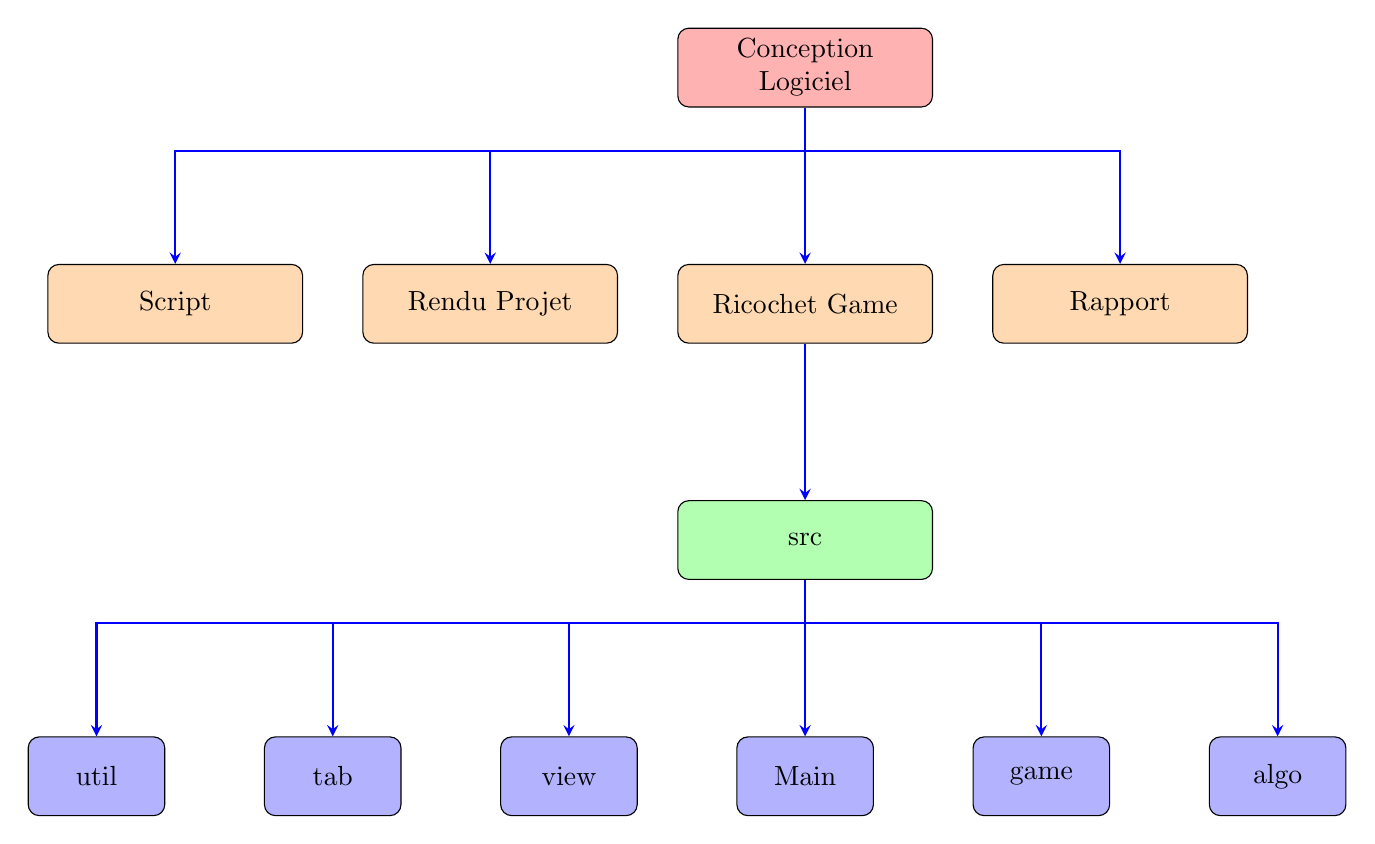
\begin{tikzpicture}[node distance=3cm]
		\node (start) [node] {Conception Logiciel} ;
		\node (RicochetGame) [level1, below of=start] {Ricochet Game};
		\node (Rapport) [level1, right of=RicochetGame, xshift = +1cm] {Rapport};
		\node (RenduProjet) [level1, left of=RicochetGame, xshift = -1cm] {Rendu Projet};
		\node (Script) [level1, left of=RenduProjet, xshift = -1cm] {Script};
		\node (src) [level2, below of=RicochetGame] {src};
		\node (main) [level3, below of=src] {Main};
		\node (game) [level3, right of=main] {game};
		\node (algo) [level3, right of=game] {algo};
		\node (view) [level3, left of=main] {view};
		\node (tab) [level3, left of=view] {tab};
		\node (util) [level3, left of=tab, xshift = 0cm] {util};
		
		\draw [arrow] (start) -- +(0,-30pt) -| (RicochetGame);
		\draw [arrow] (start) -- +(0,-30pt) -| (RenduProjet);
		\draw [arrow] (start) -- +(0,-30pt) -| (Script);
		\draw [arrow] (start) -- +(0,-30pt) -| (Rapport);
		\draw [arrow] (RicochetGame) -- +(0,-30pt) -| (src);
		\draw [arrow] (src) -- +(0,-30pt) -| (main);
		\draw [arrow] (src) -- +(0,-30pt) -|(view);
		\draw [arrow] (src) -- +(0,-30pt) -| (tab);
		\draw [arrow] (src) -- +(0,-30pt) -| (util);
		\draw [arrow] (src) -- +(0,-30pt) -| (game);
		\draw [arrow] (src) -- +(0,-30pt) -| (algo);
		\label{abr}
	\end{tikzpicture}

	\textbf{\underline{RicochetGame}}:\\
	Représente l'espace de travail.\\
	\textbf{\underline{Rapport}}:\\
	Le répertoire contenant les différents éléments du rapport.\\
	\textbf{\underline{Script}}:\\
	Contient différents scripts.\\
	\textbf{\underline{RenduProjet}}:\\
	Répertoire contenant le code à rendre.

	\subsection{\underline{Architecture du programme}}
	\subsubsection{\underline{Diaggramme des packages}}
	Le diagramme suivant est sa forme finale prise une fois que tous les éléments ont été correctement implémentés.\\
	
	\begin{figure}[h!]
		\begin{center}
			\includegraphics[width=1\textwidth]{Images/package.png}
		\end{center}
		\caption{Diagramme UML}
		\label{DU}
	\end{figure}
	Comme nous pouvons le voir le code source est décomposé en 6 packages avec le pattern \textbf{MVC} en plus pour une plus facile
	implémentation de l'interface graphique.
	\begin{itemize}
		\item Les packages \textbf{tab + game} constitue le moteur du jeu et représente le \textbf{modèle}.
		\item Le package \textbf{view} constitue la partie \textbf{vue + controlleur}
		\item Le package \textbf{algo} contient les différents solveurs.
	\end{itemize}

	%%%%%%%%%%%%%%%%%%%%%%%%%%%%%%%%%%%%%%%%%%%%%%%%%%%%%%%%%%%%%%%%%%%%%%%%%%%%%%%%%%%%%%%
	\section{\underline{Réalisation du Moteur}}
	La réalisation du moteur était la première étape que nous avions entamé et la dernière à être achevée car jusqu'au bout de 
	multiples buggs ont du être corrigés et de nouvelle fonctionalités ajoutées afin que les autres parties puissent fonctionner
	comme prévu.
	\subsection{\underline{Réalisation du Board}}
	\subsubsection{\underline{UML des classes}}
	\begin{figure}[h!]
		\begin{center}
			\includegraphics[width=1\textwidth]{Images/tab.png}
		\end{center}
		\caption{Diagramme UML du package tab}
		\label{tabuml}
	\end{figure}

	\subsubsection{\underline{Création des quartiers}}
	Pour concevoir le Ricochet Robot, la première question que nous nous sommes poser était: "comment devons-nous créer le plateau?". 
	Le plateau du Ricochet Robots est un ensemble de "mini-plateaux" qui, une fois assemblés, forment ce plateau. Dans la version 
	du jeu de société, il existe quatre morceaux de plateaux, chaque morceau ayant deux faces. Ici aussi nous avons utilisé les 
	mêmes propriétés, donnant ainsi 96 configurations de plateforme possibles.
	\\
	Pour créer le plateau, nous devions commencer par la création de ces mini-plateaux. Ces quatre mini-plateaux sont chacun 
	représenté sous la forme d'un tableau à deux dimensions, contenant des cases et des murs.\\
	Pour la réprésentation du plateau nous avons repris l'idée de Micheal Fogleman \cite{MF}, qui pour indiquer la nature de chaque case utilise 
	des caractères.\\
	\begin{lstlisting}[tabsize=2,gobble=4]
		 Q1A = {{"NW","N","N","N","NE","NW","N","N"}, 
						{"W","S","X","X","X","X","SEYH","W"},
						{"WE","NWGT","X","X","X","X","N","X"}, 
						{"W","X","X","X","X","X","X","X"},
						{"W","X","X","X","X","X","S","X"}, 
						{"SW","X","X","X","X","X","NEBQ","W"},
						{"NW","X","E","SWRC","X","X","X","S"},
						{"W","X","X","N","X","X","E","NWX"},};	
	\end{lstlisting}

	Comme nous pouvons le voir chaque case est désignée par une \textbf{chaîne de caractères(String)} représentant l'état de la case. Ici :
	\begin{itemize}
		\item \textbf{'N'} indique la présence d'un mur au nord de la case.
		\item \textbf{'S'} indique la présence d'un mur au sud de la case.
		\item \textbf{'E'} indique la présence d'un mur à l'est de la case.
		\item \textbf{'W'} indique la présence d'un mur à l'ouest de la case.
		\item \textbf{'X'} indique que la case vide.
		\item les lettres \textbf{'R', 'B', 'G', 'Y'} désignent réspectivement les couleurs des targets \textbf{red, blue, yellow, green}
		\item les lettres \textbf{'C', 'T', 'H', 'Q'} désignent respectivement la forme des targets \textbf{circle, triangle, hexagone, square} 
	\end{itemize}	
	\begin{minipage}
		
		\vspace{0.5cm}
		\begin{center}
			\begin{tikzpicture}
				\draw (1,1) rectangle (5,5);
				\draw[color=red] (1,1.5) -- (5,1.5);
				\draw[color=green] (1,4.5) -- (5,4.5);
				\draw[color=blue] (1.5,1) -- (1.5,5);
				\draw[color=olive] (4.5,5) -- (4.5,1);
				\node[color=red] (pos) at (3,0.5) {SUD};
				\node[color=green] (pos) at (3,5.5) {NORD};
				\node[color=blue] (pos) at (0,3) {OUEST};
				\node[color=olive] (pos) at (6,3) {EST};
				
				\node (posi) at (10,5) {["\textbf{NESW}" ]};
				\draw[->] (5,4) -- (posi);
			\end{tikzpicture}
		\end{center}  
		\vspace{0.5cm}
	\end{minipage}
            
            \begin{figure}[H]
                \centering
                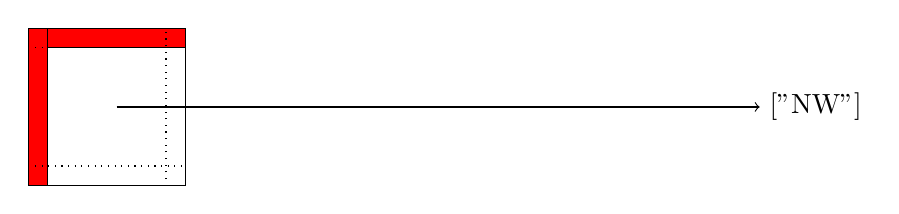
\begin{tikzpicture} 
                    \draw[fill=red] (0,2) rectangle (2, 1.75);
                    \draw[fill=red] (0,0) rectangle (0.25, 2);

                    \draw (0,0) rectangle (2,2);
                    \draw[dotted] (0,0.25) -- (2,0.25);
                    \draw[dotted] (0,1.75) -- (2,1.75);
                    \draw[dotted] (0.25,0) -- (0.25,2);
                    \draw[dotted] (1.75,0) -- (1.75,2);
                    
                    \node (void) at (1,1) {};
                    \node (str) at (10,1) {["NW"]};
                    \draw[->] (void) -- (str);
                \end{tikzpicture}
                \caption{Case ayant un mur au nord et à l'ouest}
            \end{figure}

	De cette manière nous avions obtenu une modélisation assez simple d'une face de quartier sous la forme d'une matrice de \textbf{string}.	
	Ainsi les huits faces différentes ont été formées  par la suite et chaque quartier a été affecté à deux de ces faces.	

	\subsubsection{\underline{Placement des quartiers}}
	Le plateau est composé de quatre quartiers, comme nous pouvons le voir sur la figure suivante :
	\begin{center}
		\begin{tikzpicture}
			\draw (0,0) rectangle (4,4);
			\draw[dotted] (0,2) -- (4,2);
			\draw[dotted] (2,0) -- (2,4);
			\node (4) at (1,1) {4};
			\node (3) at (3,1) {3};
			\node (2) at (3,3) {2};
			\node (1) at (1,3) {1};
		\end{tikzpicture}
	\end{center}

	Pour former à chaque fois un plateau aléatoire nous prenions au hasard l'une des faces de chaque quartier puis plaçons au hasard 
	les quartiers dans chacun des emplacements. Sauf que se limiter à ça impliquer la génération d'un tableau incorrecte, car les 
	murs de chaque quartiers devaient en plus être mises à jour.\\
	La solution adoptée fut de placer le premier quartier dans l'emplacement \textbf{Nord-Ouest} sans le changer, puis d'opérer une rotation de 90° pour
	le suivant et le placer à l'emplacement \textbf{Nord-Est}, puis une double rotation de 90° pour le troisième quatier et le placer à l'emplacement \textbf{Sud-Est}
	et enfin une triple rotation pour le dernier quatier.\\
	L'algorithme suivant \ref{algo1} montre comment marche la rotation d'un quartier et le seconde \ref{algo2} montre comment créer une grille 
	aléatoire.

	\begin{algorithm}
		\caption{ALGORITHME DE ROTATION D'UNE MATRICE}
		\SetKwInOut{Input}{Input}
		\SetKwInOut{Output}{Output}
		\Input{matrice}
		\Input{entier n réprésentant le nombre de rotation}
		\Output{matrice tournée n fois}
		\tcc{boucle sur le nombre de fois que l'on décide de tourner la matrice}
		\For{$k$ = 0; $k \leq n$; $k++$}{
			\tcc{Determiner la transposé}
			\For{$i$ = 0; $i$ < 8; $i++$}{
				\For{$j$ = 0; $j$ < 8; $j++$}{
					$tmp \gets matrice[i][j]$;\\
					$matrice[i][j] \gets matrice[j][i]$;\\
					$matrice[j][i] \gets tmp$;\
				}
			}
			\tcc{Renverser les éléments de chaque lignes}
			\For{$l$ = 0; $l$ < 8; $l++$}{
				$low \gets 0$;\\
				$high \gets 7$;\\
				\While{$low$ < $high$}{
					$tmp \gets matrice[l][low]$;\\
					$matrice[l][low] \gets matrice[l][high]$;\\
					$matrice[l][high] \gets tmp$;\\
					$low++$;\\
					$high--$;\\
				}
			}
			update(matrice);
			\tcc{fonction mettant à jour les murs}
		}
		\Return{matrice}
		\label{algo1}
	\end{algorithm}

	\begin{algorithm}[h!]
		\caption{ALGORITHME DE CREATION DE LA GRILLE 16X16}
		\SetKwInOut{Input}{Input}
		\SetKwInOut{Output}{Output}
		\Input{Tableau de taille 4 de quartiers : quartiers}
		\Output{Grille}
		$grille \gets String[16][16]$;\\
		$list \gets \emptyset$;\\
		$Q1 \gets quartiers[0].randomFace()$;\\
		$Q2 \gets quartiers[1].randomFace()$;\\
		$Q3 \gets quartiers[2].randomFace()$;\\
		$Q4 \gets quartiers[3].randomFace()$;\\
		list.add(Q1); list.add(Q2); list.add(Q3); list.add(Q4);\\
		list.\textbf{shuffle()};\\
		\For{$i$ = 0; $i \leq 3$; $i++$}{
			rotationMatrice(list.get(i),i);
		}
		\For{$i$ = 0; $i$ < 8; $i++$}{
				\For{$j$ = 0; $j$ < 8; $j++$}{
					\tcc{placement Nord-Ouest}
					$grille[i][j] \gets list.get(0)[i][j]$;\\
					\tcc{placement Nord-est}
					$grille[i][j+8] \gets list.get(1)[i][j]$;\\
					\tcc{placement Sud-est}
					$grille[i+8][j+8] \gets list.get(2)[i][j]$;\\
					\tcc{placement Sud-Ouest}
					$grille[i][j+8] \gets list.get(3)[i][j]$;\\
				}
		}
		\Return{grille}
		\label{algo2}
	\end{algorithm}
	
	\newpage
	\subsection{\underline{Fonctionnement du moteur}}
	Une fois la grille générée, nous nous sommes pencher sur le coeur de l'application c'est à dire le moteur du jeu dont la majorité
	des fonctionalités appartiennent à la classe \textbf{State} qui également joue le rôle de modèle dans l'architecture \textbf{MVC}.
	\subsubsection{\underline{Diaggramme UML}}
	\begin{figure}[h!]
		\begin{center}
			\includegraphics[width=1\textwidth]{Images/model.png}
		\end{center}
		\caption{Diagramme UML du package game}
		\label{gameuml}
	\end{figure}
	\subsubsection{\underline{Description}}
	La classe \textbf{State} donne l'état du jeu à tout instant donné. Elle initialise le jeu en créant et en plaçant les robots
	à des positions aléatoires, de même elle choisit aléatoirement une target parmis les 16 présentes sur le plateau.\\
	Elle assure les différents mouvements des robots grâces aux méthodes : 
	\begin{itemize}
		\item \textbf{possibleMove} prenant en argument un \textbf{robot et une direction} et retournant la \textbf{coordonnée finale} d'arrivée.
		\item \textbf{moveRobot} prenant un move et modifiant la position du robot.
		\item \textbf{moveRobot2} faisant la même opération que moveRobot mais retournant un nouvel état, fonction essentielle pour l'agorithme \textbf{A*}.
		\item \textbf{getValidMoves} retournant l'ensemble des moves possibles pour l'ensemble des robots, également essentielle pour \textbf{A*}. Elle fonctionne de la 
				manière suivante :
	\end{itemize}
	\begin{algorithm}
		\caption{ALGORITHME RETOURNANT L'ENSEMBLE DES MOVES POSSIBLES}
		\SetKwInOut{Input}{Input}
		\SetKwInOut{Output}{Output}
		\Input{Tableau des robots}
		\Output{List des moves possibles pour les 4 robots}
		$listOfMoves \gets \emptyset$\\
		$directions \gets \{$'N'$, $'S'$, $'E'$, $'W'$\}$;\\
		\ForEach{robot in listOfRobots}{
			\ForEach{direction in directions}{
				$coordFinal \gets possibleMoves(robot,dir)$;\\
				\If{robot.coord \textbf{not equal to} coordFinal}{
					$move = new Move(robot, coordFinal)$;
					$listOfMoves.add(move)$;
				}
			}
		}
		\Return{listOfMoves}
		\label{algoVM}
	\end{algorithm}
	\newpage

	%%%%%%%%%%%%%%%%%%%%%%%%%%%%%%%%%%%%%%%%%%%%%%%%%%%%%%%%%%%%%%%%%%%%%%%%%%%%%%%%%%%%%%%
	\section{\underline{ALGORITHME A*}}
	\subsection{\underline{Présentation}}

    L'algorithme A*\cite{WikiAstar} est un algorithme qui, à partir d'un état initial et d'un état final, permet de trouver le chemin le 
	plus court sur une carte, un plateau, etc.Il est souvent utilisé grâce a sa complétitude, son optimisation et 
	son efficience.
	La recherche de chemin s'effectue dans un graphe. Dans ce domaine, l'algorithme A* est 
	un des algorithmes les plus efficaces. Il s'agit d'un algorithme qui est relativement rapide et s'il est bien optimisé, permet de 
	trouver très rapidement la bonne solution. \\
	Il est également qualifié d'algorithme \textbf{Best-First-Search} car trouvant toujours la meilleure solution en premier.

	Il a quand même un défaut qui est sa \textbf{compléxité en espace} car il garde en mémoire tous les noeuds/états générés.

	Il existe d'autres algorithmes de recherche rapides et populaires tel que celui de recherche en profondeur \textbf{Breadth-First-Search(BFS)} \cite{WikiBFS}
	ou encore \textbf{Dijkstra} \cite{WikiDijkstra} qui peut être considéré comme le grand frère de A*.
    
	A* fonctionne en maintenant un arbre des trajets originant de la racine(le point de départ) et explorant ces trajets un à un jusqu'à
	satisfaire sa condition terminale.\\
	A chaque itération de sa boucle principale A* doit déterminer quel trajet il doit explorer. Il le fait en se basant sur le coût 
	de ce chemin qui est une estimation du coût requis pour explorer ce chemin jusqu'au point d'arrivé. Plus précisément A* choisit le 
	chemin qui minimisera :
	\begin{equation}
		f(n) = g(n) + h(n)
	\end{equation}
	Avec \textbf{n} étant le noeud suivant à explorer, \textbf{g(n)} le coût du trajet  à partir du départ jusqu'à n(\textbf{gScore}) et \textbf{h(n)} l'heuristique qui estime
	le coût du chemin de n jusqu'à l'arrivée.\\
	
	\begin{figure}[h!]
		\centering
		\includegraphics[width = 0.8\textwidth]{Images/fn.png}
		\caption{Formule de calcul du coût(\textbf{fScore})}
		\label{eq1}
	\end{figure}

	A* s'arrête lorque le trajet qu'il choisit d'explorer est celui du départ à l'arrivée ou lorsqu'il n'y a plus d'autres possibilités de chemins.\\
	La fonction heuristique varie en fontion du type de problème. Si la fonction est admissible c'est à dire qu'elle ne surestime pas le coût pour 
	atteindre l'arrivée alors A* retournera toujours le chemin le moins coûteux.
	\begin{figure}[h!]
		\centering
		\includegraphics[width = 0.8\textwidth]{Images/aStar.png}
		\caption{Problème de parcours}
	\end{figure}	
	
	\newpage
	\begin{figure}[h!]
		\centering
		\includegraphics[width = 0.4\textwidth]{Images/solution.png}
		\caption{Solution}
	\end{figure}

	Pour des explications plus en détailles et plus démonstratives nous recommendons la video de 
	\href{https://www.youtube.com/watch?v=ySN5Wnu88nE}{\textbf{Computerphile}} parlant de A* sur youtube. Elle fut d'une grande aide afin de 
	pouvoir cerner le fonctionnement l'algorithme.
%%%%%%%%%%%%%%%%%%%%%%%%%%%%%%%%%%%%%%%%%%%%%%%%%%%%%%%%%%%%%%%%%%%%%%%%%%%%%%%%%%%%%%%	
	\newpage
	\subsubsection{\underline{UML}}
	\begin{figure}[ht!]
		\centering
		\includegraphics[width = 0.8\textwidth]{Images/algo.png}
		\caption{UML du package Algo}
		\label{eq1}
	\end{figure}

	\subsection{\underline{Implémentation par rapport à Ricochet Robot}}
	L'implémentation de A* s'est faite en trois étapes.
	\begin{itemize}
		\item La première étape avec l'algorithme ne prenant en compte que les mouvements du robot
		qui avait la même couleur que la cible.(\textbf{robot actif})
		\item La deuxième étape avec l'utilisation d'une heuristique plus appropriée.
		\item Et finalement la version finale en prenant en compte l'ensemble des robots. 
	\end{itemize}  

	\subsubsection{\underline{Première Version Astar}}
	\textbf{AStar} comporte la majeur partie des décisions d'optimisation et de conception. \\
	Parlons d'abord de pourquoi nous ne faisions bouger qu'un seul robot.\\
	En effet au début à partir de toutes les documentations lues et exemples d'applications de A* étudiés, l'algorithme prenait toujours un seul
	objet situé en un point donné et cherchait à trouver le plus court chemin afin d'atteindre l'objectif. Sauf que dans notre problème
	la solution ne limite pas toujours qu'aux mouvements d'un seul robot mais plutôt des 4. En effet bouger qu'un seul robot ne garantit que une 
	fois sur trois(grosse approximation) d'arriver à la cible. Les autres robots doivent être utilisés comme obstacles afin d'aider à arriver à
	la cible.\\
	Le problème venait de là. Comment donc dire à l'algorithme de prendre en compte \textbf{les autres robots}? Solution qui ne sera apportée que par
	la dernière version.\\
	Durant l'implémentation de A* plusieurs choix d'optimisation ont été pris dont certains involontairement.\\
	Dés le début nous comptions utiliser une PriorityQueue comme choix de strucuture de données car recommender en CM et dans la plupart des articles parlant de A*.
	En effet la priorityQueue dispose d'un comparateur permettant d'ordonner les éléments de la queue. Ici notre comparateur
	était fait en sorte de mettre en tête le noeud dont le score etait le plus petit, score désignant ici $f(n) = g(n) + h(n)$ \ref{eq1}.\\
	Ainsi nous avions directement accès au meilleur noeud en temps constant. L'utilisation d'un PriorityQueue donne un gain énorme en perfomance
	comparée à une liste ou il aurait d'abord fallut chercher le meilleur élement dans la liste(temps linéaire), le récupérer puis le supprimer(temps linéaire). Tandis que pour la
	queue nous pouvons à la fois avoir accès et supprimer l'élément en temps logarithmique(voir figure ci dessous \ref{struct}).\\
	Les valeurs suivantes ont été directement prise à partir de \textbf{Github} \cite{bigO}.
	\begin{figure}[h!]
	\begin{tabular}{||p{4cm}|>{\centering\arraybackslash}p{2cm}|>{\centering\arraybackslash}p{2cm}|>{\centering\arraybackslash}p{2cm}|>{\centering\arraybackslash}p{2cm}||}
		\hline
			\rowcolor{blue!50}
			List & Add & Remove & Contains & Get\\
		\hline
			ArrayList & $\mathcal{O}$(1) & $\mathcal{O}$(n) & $\mathcal{O}$(n) & $\mathcal{O}$(1)\\
			LinkedList & $\mathcal{O}$(1) & $\mathcal{O}$(1) & $\mathcal{O}$(n) & $\mathcal{O}$(n)\\
		\hline
			\rowcolor{green!50}
			Queue & Add & Remove & Poll & Peek\\
		\hline
			PriorityQueue & $\mathcal{O}$($\log$n) & $\mathcal{O}$(n) & $\mathcal{O}$($\log$n) & $\mathcal{O}$(1)\\	
		\hline
	\end{tabular}	
	\caption{List vs Queue}
	\label{struct}
	\end{figure}

	Le deuxième choix de strucuture de donnée fut l'utilisation d'un \textbf{HashSet} afin de garder en mémoire les noeuds déjà visité pour ne 
	pas avoir à les revisiter, choix qui était un total hasard sans aucune réflexion au préalable, mais qui s'est avéré être à la fois excellent et un vrai 
	casse tête(nous y reviendrons plus tard). En effet vérifier qu'un noeud appartient au Set se fait en temps constant($\mathcal{O}(1)$).
	
	\subsubsection{\underline{Deuxième version AStarMax}} 
	\textbf{AstarMax} hérite de \textbf{Astar} et fait la même chose. La seule différence entre les deux est l'\textbf{heuristique}.
	En effet après un long de temps de recherche nous nous sommes dit que peut être une meilleure heuristique réglerai tous nos soucis. La première version
	utilisait comme heuristique une \textbf{distance de Manhattan} plus facile et rapide à calculer que la distance euclidiènne mais qui n'est pas 
	optimale comme estimation. En effet l'éloignement du robot par rapport à la cible n'a aucun rapport avec le nombre de coups nécessaire pour l'atteindre.\\
	La nouvelle heuristique consistite en un tableau de même dimension que le plateau du jeu et chaque cellule de ce tableau contient le nombre de 
	coups necessaire pour atteindre la cible à partir de cette position en assumant les autres robots étant idéalement placés.\\
	Cette idée nous est venu de Randycouleman \cite{heurist} qui lui même s'est inspiré de Micheal Fogleman \cite{MF}.
	\begin{figure}[h!]
		\centering
		\includegraphics[width=0.5\textwidth]{Images/mapHeuristique.PNG}
		\caption{Table des heuristiques}
	\end{figure}

	La création de la table fonctionne de la manière suivante:
	\begin{itemize}
		\item Mettre \textbf{1} sur toutes les cases pouvant atteindre la cible en un mouvement.
		\item Mettre \textbf{2} sur toutes las cases vides et pouvant atteindre une case contenant \textbf{1} en un mouvement.
		\item Mettre \textbf{3} sur toutes las cases vides et pouvant atteindre une case contenant \textbf{2} en un mouvement.
		\item Mettre \textbf{4} sur toutes las cases vides et pouvant atteindre une case contenant \textbf{3} en un mouvement.\\
		Ainsi de suite.
	\end{itemize}
	Cette méthode a pour avantage de limiter grandement le nombre de calculs. En effet le tableau est généré une fois au début, puis 
	à chaque fois que l'on a besoin de connaitre l'heuristique il nous suffit de récupérer la valeur de la case correspondant aux 
	coordonnées du robot \textbf{actif}(celui qui doit atteindre la cible).

	\subsubsection{\underline{Dernière version AstarFinalForm}} 
	Cette dernière version appelée \textbf{AstarFinalForm} reprend tous les 
	éléments des deux précédentes et rajoute la prise en compte des autres robots.\\
	Premièrement nous ne représentons un état comme étant uniquement la position de ses 4 robots. Ainsi un état est représenté par un
	tableau de taille 4 de coordonnées.\\
	Ensuite l'état de départ est affecté avec un score équivalent au nombre de mouvements nécessaires pour le robot actif d'atteindre la cible.
	Puis nous rajoutons cette état au  Set de noeuds visités et à la priorityQueue.\\
	A partir de l'état de départ nous générons tous les états possibles correspondant à chaque mouvement de robot. Si un état n'a pas encore était visité 
	ou est plus avantageux que les précédents, il est rajouté à la priorityQueue, et à une HashMap en même temps que l'état qui le précéde.
	La boucle principale de l'algorithme continue tant qu'il ne tombe pas sur un état verifiant la condition que le robot est arrivé à la position
	de la cible.\\
	Les algorithmes suivants sont directement inspiré de ceux présents sur le site de Wikipedia \cite{wikiAstarEN}


	\begin{algorithm}[H]
		\caption{ALGORITHME RECONSTRUCTPATH : RETOURNANT LE TRAJET}
	    \SetKwInOut{Input}{Input}
		\SetKwInOut{Output}{Output}
		\Input{HashMap cameFrom<State,State>}
		\Input{currentState}
		\Output{ListOfStates}
		$listOfStates \gets \textbf{new}$ $List<State>()$\\
		$listOfStates.\textbf{add}(currentState)$\\
		\While{$currentState \in cameFrom.\textbf{Keys}$}{
			  $currentState \gets cameFrom.\textbf{get(currentState)}$\\
			  $listOfStates.\textbf{add}(currentState)$
		}
		\Return{listOfStates}
	
	\end{algorithm}


	\begin{algorithm}
		\caption{ALGORITHME ASTAR\_FINAL\_FORM}
		\SetKwInOut{Input}{Input}
		\SetKwInOut{Output}{Output}
		\Input{initialState, h}
		\Output{listOfStates}
		$openSet \gets \emptyset$ \\
		$priorityQueue \gets \emptyset$\\
		$gScore \gets \textbf{new}$ $map<State,Int>$ with \textbf{Default Value of +$\infty$ }\\
		$fScore \gets \textbf{new}$ $map<State,Int>$\\
		$startingState \gets initialState$\\
		$openSet.\textbf{add}(startingState)$\\
		$priorityQueue.\textbf{add}(startingState)$\\
		$gScore.\textbf{put}(startingState,0)$\\
		$fScore.\textbf{put}(startingState,h(startingState))$\\
		\While{$priorityQueue$ \textbf{is not empty}}{
			$currentState \gets priorityQueue.\textbf{poll()}$\\
			\If{$currentState.\textbf{isOver()}$}{
				\Return{reconstructPath(cameFrom, currentState)}
				}
			\tcc{On explore tous les états résultant d'un mouvement de robot}
			\ForEach{neighbor of currentState}{
				$tentativeGscore \gets gScore[currentState] + 1$\\
				\tcc{S'il est meilleur que tout ce que nous avions jusqu'a présent nous le gardons}
				\If{$tentiveGscore < gScore[neighbor]$}{
					$cameFrom[neighbor] \gets currentState$
					$gScore[neighbor] \gets tentativeGscore$
					$fScore[neighbor] \gets tentativeGscore + h(neighbor)$\\
					\If{$neighbor$ $\textbf{not in openSet}$}{
						$openSet.\textbf{add}(neighbor)$\\
						$priorityQueue.\textbf{add}(neighbor)$\\
					}
				}
			}
		}
		\tcc{openSet est vide et la target jamais atteinte}
		$print(\textbf{"NO SOLUTION"})$\\
		\Return{$\emptyset$}
	\end{algorithm}


	%%%%%%%%%%%%%%%%%%%%%%%%%%%%%%%%%%%%%%%%%%%%%%%%%%%%%%%%%%%%%%%%%%%%%%%%%%%%%%%%%%%%%%%
	\newpage
	\section{\underline{Problèmes rencontrés}}
	\subsection{\underline{A*}}
	Durant l'implémentation de A* un problème semblait être insurmontable, pendant quasiment un mois nous sommes restés bloquer dessus et à
	faillit finir par nous traumatiser.\\
	En effet l'algorithme semblait tourner à l'infini quel que soit la situation du plateau. Dans l'algorihme avant d'ajouter
	un élément à la queue nous verifions à chaque fois s'il a déjà été exploré ou pas. Pour cela nous utilisions la méthodes
	\textbf{contains()}. Pendant longtemps en aucun moment nous n'avions soupconné l'origine du problème, ce n'est que apres avoir fait un 
	\textbf{println()} de la queue que l'on s'est rendu compte que la queue grandissait à l'infini et que des noeuds déjà visités étaient 
	quand même revisités.\\
	La première solution que l'on avait adopté fut de créer une classe \textbf{NoDuplicateQueue} qui est priorityQueue qui ne prenait pas 
	double en allant redéfinir sa méthode \textbf{add()}.\\ 
	Mais même aprés cela le problème était toujours présent. Ce ne que bien plus tard que l'on
	s'est mis a soupconné la méthode \textbf{contains()}.\\ 
	On est allé lire la documentation et on s'est rendu compte que contains comparait
	les \textbf{références au lieu des valeurs}.\\ 
	A partir delà nous avons décidé de redéfinir \textbf{equals} afin de régler le problème. Mais
	à la grande suprise le problème persistait.\\ 
	Pour le contourner le problème on s'est mis à faire une boucle sur tous les éléments du Set et les comparer un à un avec l'élément que 
	l'on voulait ajouter ce qui est  lent (temps linéaire) et va l'encontre de l'utilisation d'un HashSet.\\
	C'est à ce moment que notre chargé de TP Etienne LEHEMBRE nous a expliqué l'origine du problème.\\
	En effet un HashSet vérifie si deux éléments sont égaux fait à la fois appel à la méthode \textbf{equals} et la méthode \textbf{hashcode()}.\\
	Si les deux éléments ont des codes différents, ils sont considérés comme différents. Ce qui faisait que même si on avait redéfinit
	equals() cela ne suffisait pas.\\
	Il nous a fallut donc également aussi override la méthode hascode(). Après cela le problème n'était plus. \\
	De tout le projet c'est surement la chose la plus impotante que nous avons eut à apprendre.

	\subsection{\underline{GUI}}
	Durant la mise en place de l'interface graphique, nous avons voulut ajouter un boutton qui joue automatiquement tous les moves
	renvoyés par A* en faisant une boucle sur la liste retournée, mais nous avons vite constaté que l'interface ne se mettait à jour qu'à la fin 
	de la boucle.\\
	Une fois de plus le problème semblait imcomprehensible car nous avions correctement implémenté le pattern \textbf{MVC}. Un autre boutton
	qui exige que l'on click à chaque fois pour joueur un move mettait à jour l'interface à chaque fois mais l'autre non.\\
	Une fois de plus est venu à la rescousse notre chargé de tp qui aprés investigation nous a montré que l'interface était gelée et ne reprenait 
	la main que une fois la boucle terminée.\\
	Pour résoudre le problème il a fallut faire tourner l'interface et la méthode faisant une boucle sur les moves retournés sur différents 
	\textbf{threads}. Qui fut une première car jusque là nous n'avions jamais considéré cette éventualité.\\
	La liste de problèmes rencontrés durant ce projet étant extremment longue nous nous limiterons à ces deux qui furent les plus problématiques.
	
	\newpage
	\section{\underline{Conclusion}}
	\subsection{\underline{Avis Général}}
	Ce projet était très intéressant. Nous ne connaissions pas le Ricochet Robots auparavant et c'était intéressant de se pencher, 
	sur les règles de ce jeu et de le recréer afin de pouvoir y jouer autrement que sous forme physique.\\
	Ce projet nous aura permis de beaucoup apprendre et de nous améliorer.
	
	\subsubsection{\underline{Eléments à améliorer}}
	Bien que tout ce qui a été demandé dans le sujet a été remplit, pas mal de choses restent quand même à améliorer mais faute de 
	temps et du nombre de projets à finir en ce fin semestre tout ce que l'on souhaité n'a pas pu être accomplit.
	Par exemple:
	\begin{itemize}
		\item Amélioreration de  l'interface graphique, car l'interface finale est trés basique.
		\item Rajouter d'autres fonctionnalités comme pourvoir jouer par soi même.
		\item Faire des tests comparant différents type d'algorithmes.
	\end{itemize}

	\newpage
\bibliographystyle{unsrt}
\bibliography{bibliography}


\end{document}
